\newpage
\section{Theoretical Analysis}
\label{sec:analysis}
In this section, the circuit shown in Figure~\ref{fig:Circuit} is analysed
theoretically. \\
\noindent As already mentioned, the audio amplifier is a circuit with two different stages: the gain stage, in which the voltage input signal is amplified, and the output stage, in which the output impedance is low, so the circuit can be connected to a speaker, while the signal degradation is minimized. In the first stage, the purpose is to have the higher possible gain and the degradation of the signal is avoided with a high input impedance. In the transition between the two stages, the degradation is also prevented, since the input impedance in the second stage is lower than the output impedance of the gain stage, because of the way the two sub-circuits are connected. Finally, in the output stage, the goal is not to amplify the signal, but it should not be attenuated either- this is well achieved since the gain is very close to 1.\\ 
\noindent The incremental circuit used to compute gain, input and outuput impedances is shown in Figure~\ref{fig:Incremental}.

\begin{figure}[h!] \centering
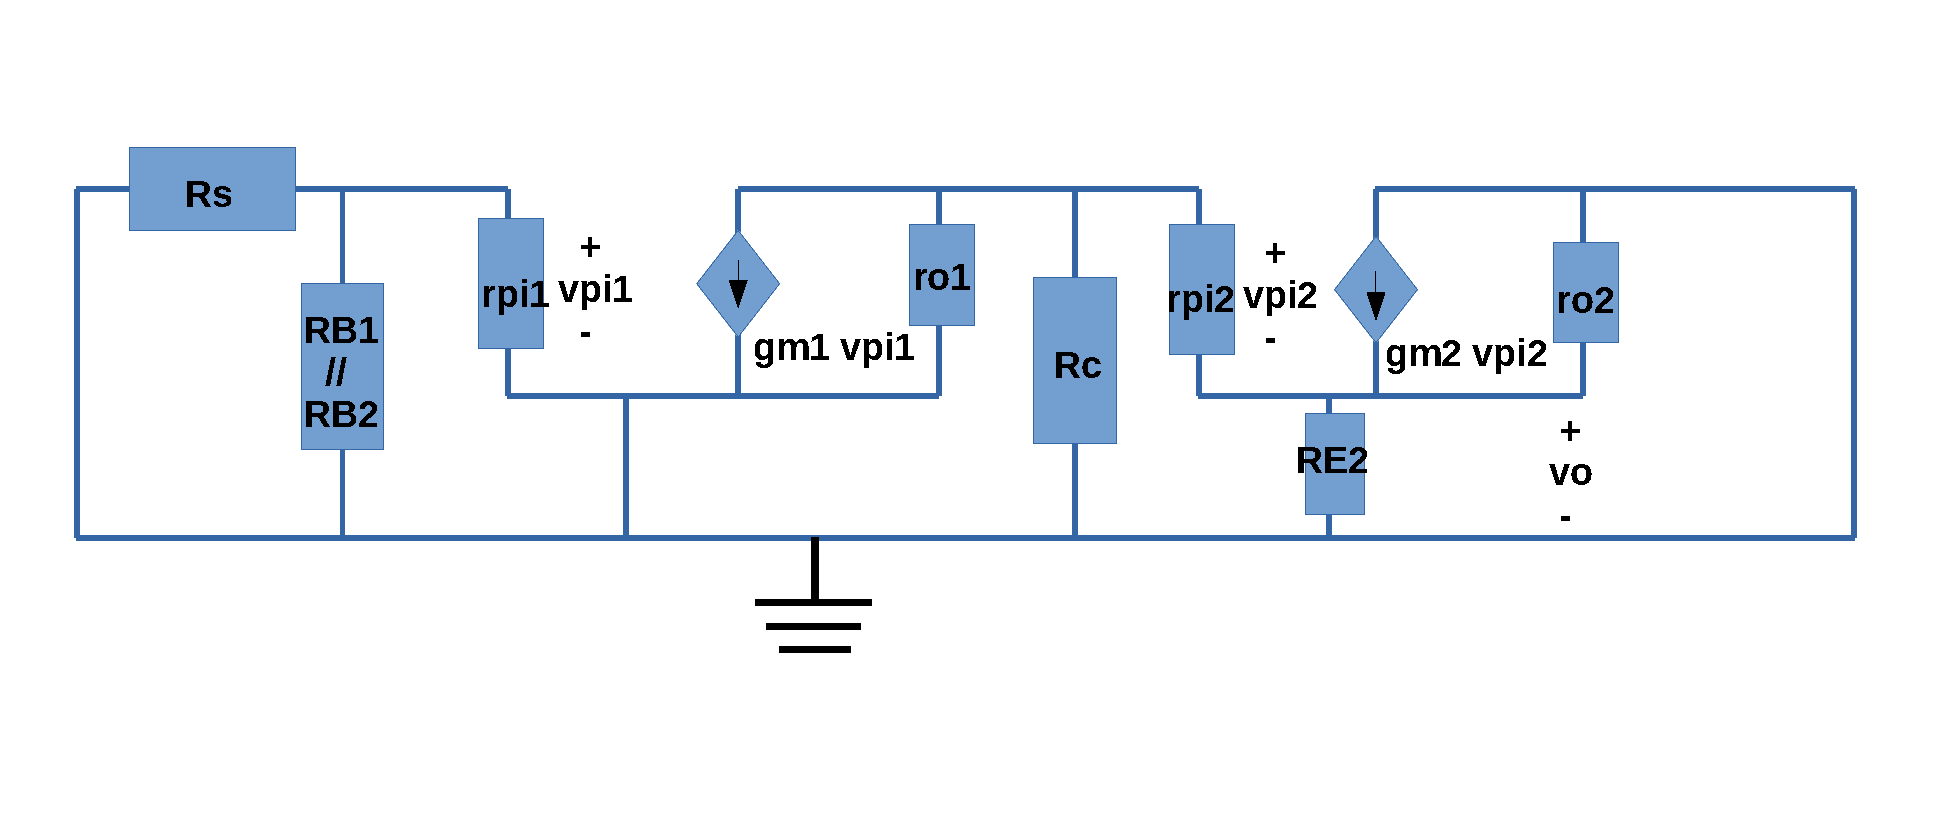
\includegraphics[width=0.8\linewidth]{Incremental.pdf}
\caption{Incremental circuit.}
\label{fig:Incremental}
\end{figure}

The values used for the parametres are showed in the following table:

\begin{table}[!h]
\centering
\begin{small}
\caption{Values of the circuit parameters} \label{Table1}
\begin{tabular}{|c|c|}
\hline
$n_{transistors}$  & \partialinput{1}{1}{tabelaVal.tex}\\
$C_i$   & \partialinput{2}{2}{tabelaVal.tex} \\
$C_b$   & \partialinput{3}{3}{tabelaVal.tex} \\
$C_o$    & \partialinput{4}{4}{tabelaVal.tex} \\
$RE1$    & \partialinput{5}{5}{tabelaVal.tex} \\
$RE2$    & \partialinput{6}{6}{tabelaVal.tex} \\
$RC$    & \partialinput{7}{7}{tabelaVal.tex} \\
$RB1$    & \partialinput{8}{8}{tabelaVal.tex} \\
$RB2$    & \partialinput{9}{9}{tabelaVal.tex} \\
$RS$    & \partialinput{10}{10}{tabelaVal.tex} \\
\hline
\end{tabular}
\end{small}
\end{table}

\subsection{Gain Stage}
\label{sec: gain}
\noindent The circuit used in the gain stage uses a capacitor $C_{E}$ to bypass the resistor ${R_E}$. To simplify, we consider that $C_{E}$ behaves like a short-circuit for high frequencies (AC current) and as an open-circuit for low frequencies (DC current). In AC, the current only flows through the short-circuit (since it has 0 impedance), improving the gain. In DC, the current only flows through the resistor (since it cannot flow through an open-circuit), which stabilizes the temperature effect. 
\noindent The first step of the theoretical analysis is to compute the operating point using the DC model. To do that we used the expressions below:
\begin{equation}
	 R_{B}= \frac{1}{ R_{B1}||R_{B2} }
	\label{eq:R_B}
\end{equation}
\begin{equation}
	 V_{EQ} = \frac{{R_{B2}}{V_{CC}}}{R_{B1}+R_{B2}}
	\label{eq:V_EQ}
\end{equation}
\begin{equation}
	I_{B1}= \frac{V_{EQ}-V_{BEON}}{R_{B}+{1+B_{FN}}{R_{E1}}}
	\label{eq:I_B1}
\end{equation}
\begin{equation}
	I_{C1}= {B_{FN}}{I_{B1}}
	\label{eq:I_C1}
\end{equation}
\begin{equation}
	I_{E1}={1+B_{FN}}{I_{B1}}
	\label{eq:I_E1}
\end{equation}

\begin{equation}
	V_{E1} = {R_{E1}}{I_{E1}}
	\label{eq:V_E1}
\end{equation}
\begin{equation}
	V_{O1}=V_{CC}-{R_{C1}}{I_{C1}}
	\label{eq:V_O1}
\end{equation}
\begin{equation}
V_{CE}= V_{O1}-V_{E1}
	\label{eq:V_CE}
\end{equation}
 
\noindent We have verified that both BJTs are in the Forward Active Region. The condition considered for that purpose was, for the NPN transistor: $V_{CE} > V_{BE} <=> V_{C} > V_{B}$ and for the PNP transistor: $V_{EC} > V_{EB} <=> V_{C} < V_{B}$
\noindent Next, we can compute the gain, input and output impedances separately for the 2 stages, using the incremental analysis. For the first stage, we use the following expressions to calculate such parameters.
\begin{equation}
	Gain_{1} = - {g_{m1}}{r_{o1}||R_{c}} {\frac{R_{B}||r_{pi}}{R_{B}||r_{pi1}+R_{s}}} 
	\label{eq:gain_stage_gain}
\end{equation}
\begin{equation}
	Z_{in1} = R_{B} || r_{pi1}
	\label{eq:gain_stage_input_impedance}
\end{equation}
\begin{equation}
	Z_{out1} = r_{o1} || R_{C}
	\label{eq:gain_stage_output_impedance}
\end{equation}

\subsection{Output Stage}
\label{sec: output}
For the second stage, we analysed the operating point using the following equations:
\begin{equation}	
V_{I2} = V_{O1}
	\label{eq:V_I2}
\end{equation}
\begin{equation}	
I_{E2} = \frac{V_{CC}-V_{EBON}-V_{I2}}{R_{E2}}
	\label{eq:I_E2}
\end{equation}
\begin{equation}	
I_{C2} = \frac{{B_{FP}}{I_{E2}}}{B_{FP}+1}
	\label{eq:I_C2}
\end{equation}
\begin{equation}	
V_{O2} = V_{CC} – {R_{E2}}{I_{E2}}
	\label{eq:V_O2}
\end{equation}

By inspection of the circuit, we can see that the voltage of the base is equal to Veq (since there is no current passing through the resistor at the DC model- C is an open-circuit); the voltage in the collector of the gain stage is equal to Vout1 (since it connects the collector to the ground); for the same reason, the voltage in the emitor of the output stage is equal to Vout2; the input voltage of the gain stage is AC, hence in the operating point model it is seen as 0; the voltage in2 is 0 too, since there is no current flowing through the resistor, as explained before; finally, the output voltage in DC analysis is 0, since the capacitor is replaced with a short-circuit, which means that there is no current flowing through the resistor. All this values are summarized in the table bellow.

\begin{table}[!h]
\centering
\begin{small}
\caption{Operating Point: Node Voltages(V)} \label{Table4}
\begin{tabular}{|c|c|}
\hline
$base$  & \partialinput{1}{1}{tabelaN.tex}\\
$coll$   & \partialinput{2}{2}{tabelaN.tex} \\
$emitter1$   & \partialinput{3}{3}{tabelaN.tex} \\
$emitter2$    & \partialinput{4}{4}{tabelaN.tex} \\
$in$    & \partialinput{5}{5}{tabelaN.tex} \\
$in2$    & \partialinput{6}{6}{tabelaN.tex} \\
$out$    & \partialinput{7}{7}{tabelaN.tex} \\
$Vcc$    & \partialinput{8}{8}{tabelaN.tex} \\
\hline
\end{tabular}
\end{small}
\end{table}

\noindent Using the incremental circuit in Figure~\ref{fig:Incremental}, we have computed gain, input and output impedances, for this stage, using the expressions below:
\begin{equation}
	Gain_{2} = \frac{g_{pi2}+g_{m2}}{g_{pi2}+g_{o2}+g{E2}+g_{m2}}
	\label{eq:output_stage_gain}
\end{equation}
\begin{equation}
	Z_{in2} = \frac{r_{pi2}}{1- \frac {g_{pi2}+g_{m2}} { g_{pi2}+ g_{o2}+ g_{E2}+ g_{m2}}}
	\label{eq:output_stage_input_impedance}
\end{equation}
\begin{equation}
	Z_{out2} = \frac{1}{g_{m2}+ \frac{1}{r_{o2}}+ \frac{1}{R_{E}}+ \frac{1}{r_{pi2}}}
	\label{eq:output_stage_output_impedance}
\end{equation}


\noindent Calculating the values of the previous expressions, for both gain and output stage, the following table is obtained:

\begin{table}[!h]
\centering
\begin{small}
\caption{Results obtained for stages separately} \label{Table2}
\begin{tabular}{|c|c|}
\hline
$Gain (Gain Stage)$  & \partialinput{1}{1}{tabela2.tex}\\
$Imput Impedance (Gain Stage)$   & \partialinput{2}{2}{tabela2.tex} \\
$Output Impedance (Gain Stage)$   & \partialinput{3}{3}{tabela2.tex} \\
$Gain (Output Stage)$  & \partialinput{4}{4}{tabela2.tex}\\
$Imput Impedance (Output Stage)$   & \partialinput{5}{5}{tabela2.tex} \\
$Output Impedance (Output Stage)$   & \partialinput{6}{6}{tabela2.tex} \\
\hline
\end{tabular}
\end{small}
\end{table}

\subsection{Total circuit}
\label{sec: total}
To complete the last task, we analysed the incremental circuit above. The goal is to compute the total gain as a function of the frequency. To do that we need to compute the cut off frequencies. Since the upper cut off frequency is too high to be evaluated in the considered problem, we can assume it as infinity, since it is not in the range of audible frequencies, from 20Hz to 20kHz. The lower cut off frequency was calculated as a function of the capacitances of the capacitors, considering that for each equivalente impendance that the others capacitors are short-circuits:
\begin{equation}
	lco = \frac{1}{2pi}({ \frac{1}{{ZO}{Co}} + \frac{1}{{ZI}{Ci}} + \frac{1}{{Zb}{Cb}}})
	\label{eq:lower_cut_off_frequency}
\end{equation}
\noindent For frequencies bellow the lower cut off frequency, we considered a linear relation between the gain and the frequency with a slope of 20 dB per decade. Once this frequency is achieved, the graph is constant since we considered the higher cut off frequency as infinite. The only unknown variable by now is that constant value, which can be calculated with the following expression, in which $Gain_{1}$ is the value obtained in equation~\ref{eq:gain_stage_gain}.  

\begin{equation}
	A_{V} = {\frac{g_{B}+\frac{{g_{m2}}{g_{B}}}{g_{pi2}}}{g_{B}+g_{e2}+g_{o2}+ \frac{{g_{m2}}{g_{B}}}{g_{pi2}}}}{Gain_{1}}
	\label{eq:gain_between_the_cut_off_frequencies}
\end{equation}
\noindent The following plot shows the frequency response of the total circuit.

\begin{figure}[h!] \centering
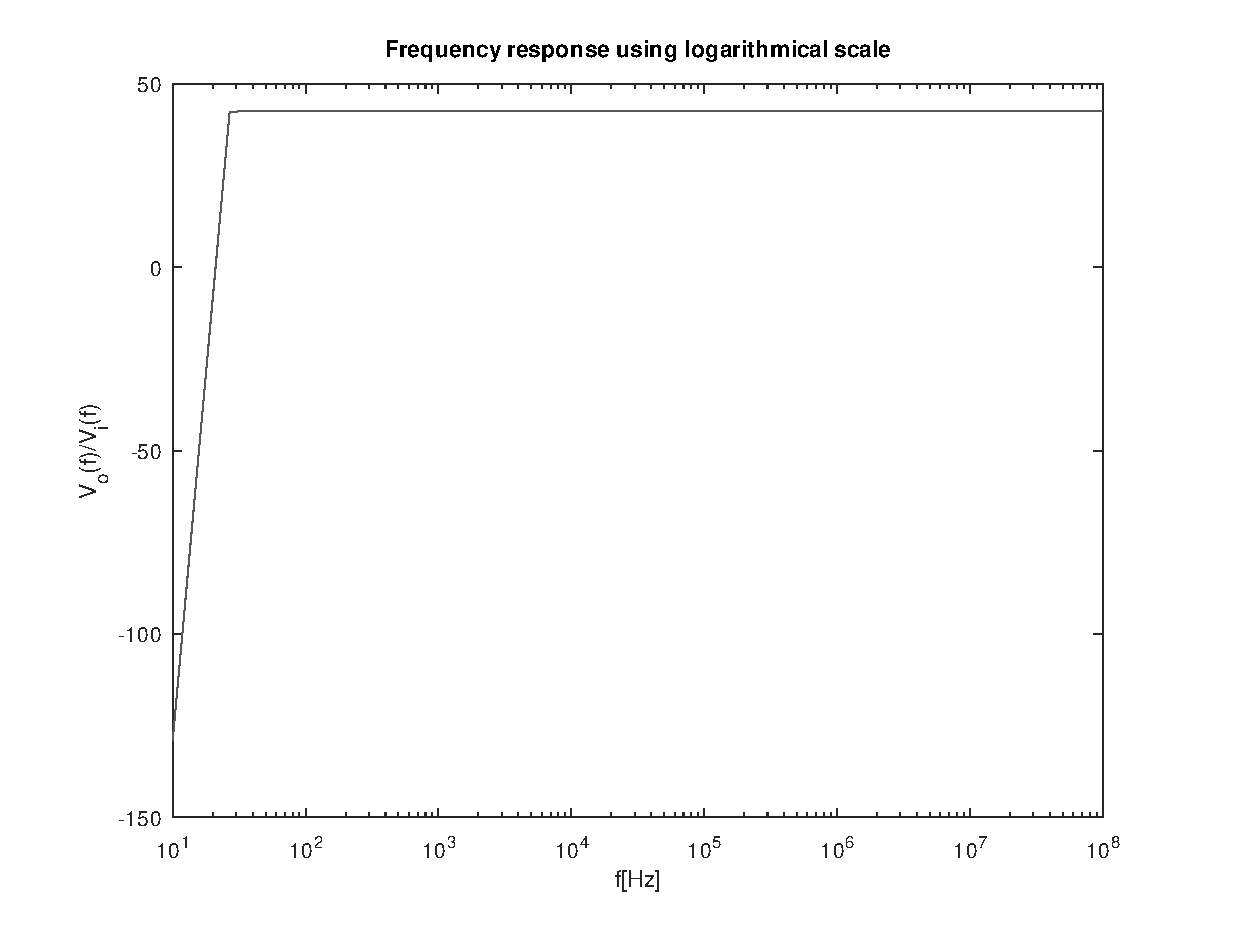
\includegraphics[width=0.7\linewidth]{plot1.eps}
\caption{Frequency response.}
\label{fig:FR}
\end{figure}

\noindent It is evident that the input impedance of the total circuit is the same as for the gain stage, since the input voltage is not connected to the output stage. So, the last unknown we need to compute is the total output impedances, for which we used the following expression:
\begin{equation}
	Z_{Ototal} = \frac{1}{ g_{o2} + \frac{{g_{m2}}{g_{B}}}{g_{pi2}} + g_{e2}+g_{B}}
	\label{eq: Total output impedance}
\end{equation}


\noindent Since we considered the upper cut off frequency as infinity, the bandwidth is also infinity, therefore, for the theoretical analysis it makes no sense to calculate the merit value.
\noindent Finally, the following table presents the theoretical obtained results for: total circuit gain, lower cut off frequency, bandwidth, cost, input and output impedances.

\begin{table}[!h]
\centering
\begin{small}
\caption{Results obtained} \label{Table3}
\begin{tabular}{|c|c|}
\hline
$TotalGain$  & \partialinput{3}{3}{tabelaRes.tex}\\
$LowerCutoffFrequency$   & \partialinput{2}{2}{tabelaRes.tex} \\
$Bandwidth$   & $\infty$ \\
$cost$    & \partialinput{1}{1}{tabelaRes.tex} \\
$ImputImpedance$    & \partialinput{4}{4}{tabelaRes.tex} \\
$OutputImpedance$    & \partialinput{5}{5}{tabelaRes.tex} \\
\hline
\end{tabular}
\end{small}
\end{table}




